\section{Data and System Architecture}

\subsection{Recorded streams}

The primary research dataset is Binance spot BTCUSDT. Two independent streams
are recorded into hourly gzip-compressed JSON Lines files:

\begin{itemize}
  \item depth diffs plus periodic 1,000-level REST snapshots; and
  \item aggregate trades, including exchange trade time, aggregate trade ID,
        price, quantity, and the buyer-maker flag.
\end{itemize}

Depth quantity zero removes a price level; a nonzero quantity replaces the
aggregate displayed quantity at that level. Snapshots establish a new
\code{lastUpdateId}. Diffs at or before that ID are discarded, and replay
resumes only when the first retained diff satisfies the exchange bridge
condition \citep{binancews2026,binancerest2026}. Depth diffs expose Binance
event time \code{E}; aggregate trades expose matching time \code{T}. REST
snapshots have no exchange event timestamp.

The legacy recorder stamped each snapshot with request-start/rotation time
before its blocking REST fetch completed. Frozen V2 replay applied the returned
book at that early tag. The current recorder persists request and response times
separately. Under \code{post_response_proxy_depth_boundary_v1}, replay emits a
fail-closed barrier at recorded local request time, then establishes a valid
bridge and requires a sequence-valid retained depth receipt after response
completion. Legacy files use the first strictly later receipt as a post-response
upper-bound proxy. Reconstruction is released at the selected record's \code{E},
and only its final state reaches strategy logic. Local request time, depth
\code{E}, trade \code{T}, and receipt times retain different semantics and
uncalibrated latency; this is not a calibrated observation clock.

Perpetual-futures depth and raw trade capture also exists, isolated in separate
directories so its schema cannot collide with spot. That dataset remains
recording-only: this report makes no spot--perpetual comparison.

\subsection{Integrity inventory and panel selection}

The frozen manifest inventories \ManifestHours\ hourly slots before 1 June
2026. Of these, \ManifestValidHours\ passed the required file, gzip, JSON,
snapshot-bridge, and sequence checks; \ManifestInvalidHours\ did not. Most
failures reflect missing recorder files, with some decode or sequence issues.
Any five-hour window containing an invalid hour was ineligible.

Development selection retained the six exploratory anchors and filled the
panel with non-overlapping valid windows while balancing UTC buckets and
one-second realized-volatility terciles. The result is \DevelopmentWindows\
development windows and \HoldoutWindows\ holdout windows. Development is
concentrated in 12--20 April and 6--9 May; the holdout is in late May. Clean
recording is therefore not assumed to be missing completely at random. If feed
or recorder failure correlates with stressed markets, eligibility can itself
select the sample.

\begin{figure}[H]
  \centering
  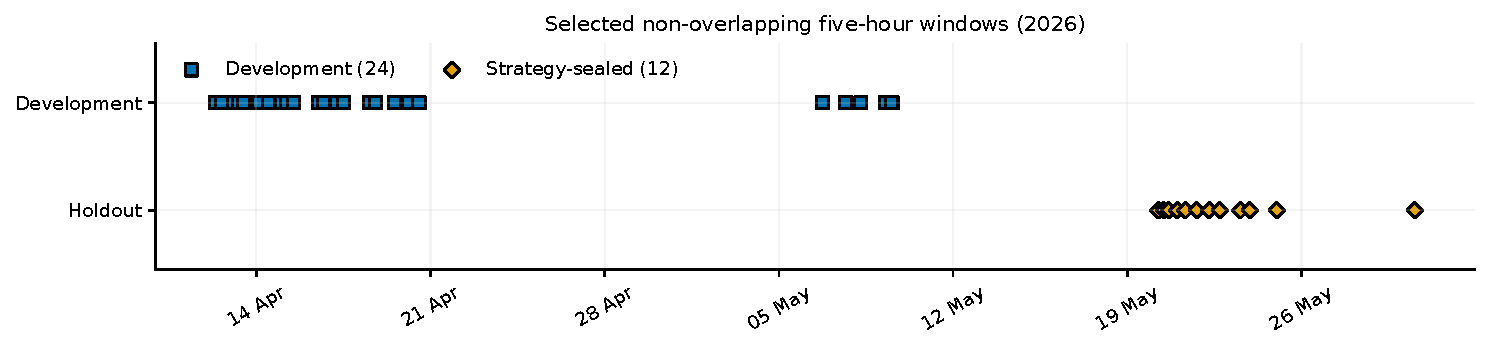
\includegraphics[width=0.96\textwidth]{figures/panel_timeline.pdf}
  \caption{Frozen selected panel. The holdout is strategy-sealed, not unseen:
  window identities and pre-strategy descriptors were examined, but no
  candidate strategy was evaluated on them. The regime comparison
  labels the holdout \emph{regime-shifted}, principally because realized
  volatility and jump counts were lower.}
  \label{fig:panel-timeline}
\end{figure}

The full integrity identity begins \texttt{\ManifestHashShort}; the selected
panel identity begins \texttt{\PanelHashShort}. Exact SHA-256 values and every
selected start are committed in the canonical artifacts.

A publication-time audit hash-checked all 120 selected development depth files.
Every snapshot bridged. The first later local depth receipt followed the legacy
tag by a median \SnapshotReceiptMedianMs{} ms, 90th percentile
\SnapshotReceiptPninetyMs{} ms, and maximum \SnapshotReceiptMaxMs{} ms. This is
an upper-bound response-completion proxy, not a measured round trip. Frozen
fills associated with orders placed before the selected policy boundary numbered
\SnapshotPreBridgeFillsQcZero{} at $c=0$ and
\SnapshotPreBridgeFillsQcOne{} at $c=1$. This is a proxy diagnostic, not an upper
bound or a robustness result, and it cannot exclude changed queue age. In all
120 files the selected policy boundary was the valid bridge, but its replay time
remains exchange \code{E}. The full V3 panel must be rerun under the new policy.

\subsection{Data availability}

Raw recordings are not stored in Git. At the report date the complete local
multi-dataset capture is approximately 37 GB, including unused
perpetual-futures data. The two spot directories used here occupy approximately
20.5 GB; the 240 selected development files occupy approximately 0.82 GB. The
tracked repository contains only selected derived artifacts. This gives three
distinct reproducibility levels:

\begin{enumerate}
  \item a fresh clone can run deterministic unit tests and a synthetic
        event-driven lifecycle demo;
  \item a fresh clone can validate the committed artifact structure, expected
        identities and verdict fields, regenerate report figures, and confirm
        that no candidate holdout artifact exists; and
  \item reproducing replay-derived numbers requires the locally held raw files
        whose hashes are recorded in the integrity manifest.
\end{enumerate}

The repository therefore uses the precise term \emph{artifact-verifiable}; it
does not claim that the full empirical panel can be rerun from a clone alone.

\subsection{End-to-end architecture}

Figure \ref{fig:architecture} shows the main information flow. Strategies
express intent through order or cancellation requests. The execution simulator,
not the strategy, owns arrival time, order state, queue position, fills, and
fees. This boundary keeps trading logic independent of execution mechanics and
makes it possible to test the latter with synthetic event paths.

\begin{figure}[H]
\centering
\begin{tikzpicture}[
  node distance=0.72cm and 0.65cm,
  box/.style={draw=Navy, rounded corners=2pt, fill=PaleBlue, align=center,
              minimum height=1.0cm, text width=2.45cm, font=\small},
  analysis/.style={draw=BluishGreen, rounded corners=2pt, fill=PaleTeal, align=center,
                   minimum height=1.0cm, text width=2.45cm, font=\small},
  arrow/.style={-{Latex[length=2.2mm]}, thick, draw=Slate}
]
  \node[box] (raw) {Depth snapshots/diffs\\and aggregate trades};
  \node[box, right=of raw] (parse) {Gap-aware parsers\\and event merger};
  \node[box, right=of parse] (book) {Decimal L2 book\\and state hashes};
  \node[box, below=of parse] (engine) {Timestamp-batched\\replay engine};
  \node[box, left=of engine] (strategy) {Quoting strategy\\intent callbacks};
  \node[box, right=of engine] (sim) {Execution simulator\\and private scheduler};
  \node[analysis, below=of engine] (analysis) {P\&L, markout, OFI,\\queue and tail analysis};
  \node[analysis, right=of analysis] (artifacts) {Hashed artifacts, gates,\\and verification};

  \draw[arrow] (raw) -- (parse);
  \draw[arrow] (parse) -- (book);
  \draw[arrow] (parse) -- (engine);
  \draw[arrow] (book) -- (engine);
  \draw[arrow] (engine) -- (strategy);
  \draw[arrow] (strategy) -- (sim);
  \draw[arrow] (sim) -- (engine);
  \draw[arrow] (engine) -- (analysis);
  \draw[arrow] (analysis) -- (artifacts);
\end{tikzpicture}
\caption{System architecture. Recorded market data and simulated private
actions meet on the deterministic modeled clock defined in Section~4.}
\label{fig:architecture}
\end{figure}

\subsection{Component responsibilities}

\begin{table}[H]
\centering
\caption{Primary code boundaries.}
\begin{tabularx}{\textwidth}{@{}L{0.29\textwidth}Y@{}}
\toprule
Component & Responsibility \\
\midrule
\artifact{src/replay/orderbook.py} & Sorted aggregate depth, best prices and sizes, mid, spread, microprice, snapshots/diffs, deterministic state hash. \\
\artifact{src/replay/depth_parser.py} & Hourly depth decoding, snapshot bridging, stale-diff rejection, and sequence-gap propagation across files. \\
\artifact{src/replay/trade_parser.py} & Aggregate-trade decoding, modeled ordering field, aggressor side, and ID-gap detection. \\
\artifact{src/replay/event_merger.py} & Stable two-way market-data merge and the recorded depth-before-trade tie rule. \\
\artifact{src/replay/engine.py} & Timestamp grouping, book mutation, strategy callbacks, private-action scheduling, gap policy, and replay termination. \\
\artifact{src/execution/simulator.py} & Entry/cancel latency, order lifecycle, post-only checks, FIFO queue state, partial fills, volume conservation, and fees. \\
\artifact{src/strategies/base_mm.py} & Inventory and live-order tracking, tick rounding, requote behavior, and the hard working-exposure envelope. \\
\directory{src/analysis} & Markouts, P\&L decomposition, matched lots, bootstrap intervals, OFI/microprice tests, fee and queue sensitivity, and tail diagnostics. \\
\bottomrule
\end{tabularx}
\end{table}

\subsection{Determinism}

Prices, quantities, fees, queue ranks, and accounting use
\code{decimal.Decimal}. Latency jitter uses seeded independent random streams
for entries and cancels. Replay uses recorded timestamps without runtime clock
reads. Every
checkpoint hashes a canonical serialization of full book state. Determinism is
necessary for debugging, regression testing, artifact identity, and eventual
cross-language parity; it does not by itself validate the economic assumptions
of the simulator.
